\documentclass[11pt]{exam}
\usepackage{graphicx, bm, listings, txfonts, logicproof, tikz}
\title{Computational Logic - Assignment 3}
\author{Alessandro Marostica}
\date{\today}
\begin{document}
\maketitle
\section*{Exercise 2}
Let's break down the proof in two parts:
\begin{enumerate}
    \item R is symmetric \(\Rightarrow \varphi \Rightarrow \square \diamond \varphi\)
    \item \(\varphi \Rightarrow \square \diamond \varphi \Rightarrow\) R is symmetric
\end{enumerate}
\textbf{R is symmetric} \boldmath{\(\Rightarrow \varphi \Rightarrow \square \diamond \varphi\)}: \\
Let's assume that \(\varphi\) is true in a world w, \(w \vDash \varphi\). We need to show that \(w \vDash \square \diamond \varphi\).
By definition of modal operators, since R is symmetric, if v is accessible from w, then w is accessible from v. Therefore, if \(\varphi\) is true in v, then \(\varphi\) is also true in w.
This implies that \(\square \varphi\) is true in w and \(\diamond \varphi\) is true in w. Therefore \(\square \diamond \varphi\) holds in w.
Since this holds for an arbitrary world w where \(\varphi\) is true, we can conclude that \(\varphi \Rightarrow \square \diamond \varphi\). \\
\textbf{\(\varphi \Rightarrow \square \diamond \varphi \Rightarrow\) R is symmetric}: \\
To show symmetry, we need to show that if \(wRv\) then \(vRw\) for all worlds w and v.
Let's assume \(wRv\), this means that v is accessible form w.
Let's also consider the formula \(\varphi = \neg \square \neg \diamond \bot \), which is not necessarily false. By assuming \(\varphi \Rightarrow \square \diamond \varphi\), we have \(\neg \square \neg \diamond \bot \Rightarrow \square \diamond \neg \square \neg \diamond \bot\).
In the world w:
\begin{enumerate}
    \item \(\neg \square \neg \diamond \bot\) is true in w since \(\diamond \bot\) is true in vv, which is accessible from w.
    \item \(\square \diamond \neg \square \neg \diamond \bot\) is true in w by assumption.
\end{enumerate}
This implies that \(\neg \square \neg \diamond \bot\) is true in all worlds accessible from w, including v.
Now, considering formula \(\diamond \bot\), we have that this is true in v since \(\neg \square \neg \diamond \bot\) is true in v. Therefore \(vRw\).
Since this is true in an arbitrary world, we can conclude that R is symmetric.
\section*{Exercise 3}
As in Exercise 2, we will break down this proof in two parts:
\begin{enumerate}
    \item F is euclidean \(\Rightarrow F \vDash \diamond \varphi \Rightarrow \square \diamond \varphi\)
    \item \(F \vDash \diamond \varphi \Rightarrow \square \diamond \varphi \Rightarrow\) F is euclidean
\end{enumerate}
\textbf{F is euclidean} \boldmath{\(\Rightarrow F \vDash \diamond \varphi \Rightarrow \square \diamond \varphi\)}: \\
Let w be a world in W, Suppose \(w \vDash \diamond \varphi\), meaning there exists a world v such that \(wRv\) and \(v \vDash \varphi\).
We now need to show that \(w \vDash \square \diamond \varphi\). Thanks to the euclidean property, if \(wRv\) and \(wRu\) then \(vRu\) for any u in W.
Since \(wRv\) is reflexive, \(vRw\), then \(vRv\). This means that \(\diamond \varphi\) is true at v. Now \(\square \diamond \varphi\) is ture at w because \(\diamond \varphi\) is ture at all worlds accessible from w. \\
\textbf{\(F \vDash \diamond \varphi \Rightarrow \square \diamond \varphi \Rightarrow\) F is euclidean}: \\
Let's take any \(x, y, z\) in W such that \(xRy\) and \(xRz\). We need to show that \(yRz\).
Let's consider the formula \(\phi = \diamond \varphi\), where \(\phi\) is an arbitrary formula. Since \(xRy\) there exists \(u\) such that \(xRu\) and \(u \vDash \varphi\).
Now, \(xRz\) and, by assuming \(F \vDash \diamond \varphi \Rightarrow \square \diamond \varphi\), we have \(xRz \Rightarrow zRw\) for any w such that \(xRu\).
Therefore we have \(zRw\) for some w such that \(xRu\). Since y is accessible from x, y is also accessible from u, which implies \(yRw\).
Given \(yRw\) and \(zRw\), by transitiviy we have \(yRz\).
Since this holds for arbitrary \(x, y, z\) in W, we can conclude that F is euclidean.
\section*{Exercise 4}
\subsection*{Model 1}
\begin{enumerate}
    \item \(x_1 \Vdash \diamond \diamond \square \bot \)
    \item \(x_2 \Vdash (\diamond \square \bot) \wedge \neg (\diamond \diamond \diamond \square \bot) \)
    \item \(x_3 \Vdash \square \bot \)
    \item \(x_4 \Vdash \diamond \diamond \diamond \square \bot \)
\end{enumerate}
\subsection*{Model 2}
\begin{enumerate}
    \item \(x_1 \Vdash \diamond \diamond \square \bot\): \(x_1\) is the world where two jumps are needed to reach a world with no accessible neighbours.
    \item \(x_2, x_4 \Vdash \diamond \square \bot\): States 2 and 4 cannot be uniquely characterized since they can both directly reach a world with no accessible neighbours.
    \item \(x_3 \Vdash \square \bot \): \(x_3\) is the world with no accessible neighbours.
\end{enumerate}
\section*{Exercise 5}
\begin{enumerate}
    \item \begin{center}
        \(\vdash \diamond(P \rightarrow Q) \rightarrow (\square P \rightarrow \diamond Q)\)
        \begin{logicproof}{5}
            \begin{subproof}
                \diamond(P \rightarrow Q) & Assumption \\
                \neg \square \neg (P \rightarrow Q) & Rewrite 1 \\
                \begin{subproof}
                    \square P & Assumption \\
                    \begin{subproof}
                        \square \neg Q & Assumption \\
                        \begin{subproof}
                            P & \(\square e 3\) \\
                            \neg Q & \(\square e 4\) \\
                            \begin{subproof}
                                P \rightarrow Q & Assumption \\
                                Q & \(\rightarrow e 5, 7\) \\
                                \bot & \(\neg e 6, 8\)
                            \end{subproof}
                            \neg (P \rightarrow Q) & \(\neg i 7-9\)
                        \end{subproof}
                        \square \neg (P \rightarrow Q) & \(\square i 5, 10\) \\
                        \bot & \(\neg e 2, 11\)
                    \end{subproof}
                    \neg \square \neg Q & \(\neg i 4-12\)
                \end{subproof}
                \square P \rightarrow \neg \square \neg Q & \(\rightarrow i 3-13\) \\
                \square P \rightarrow \diamond Q & Rewrite 15
            \end{subproof}
            \diamond(P \rightarrow Q) \rightarrow (\square P \rightarrow \diamond Q) & \(\rightarrow i 1-15\)
        \end{logicproof}
    \end{center}
    The box from line 5 to line 10 should be dashed, yet I had no idea how to make one.
    \item \begin{center}
        \(\vdash \square (\square P \rightarrow Q) \vee \square (\square Q \rightarrow P)\)
    \end{center}
    To prove the invalidity of this sequent it is sufficient to provide such Kripke structure:
    \begin{center}
        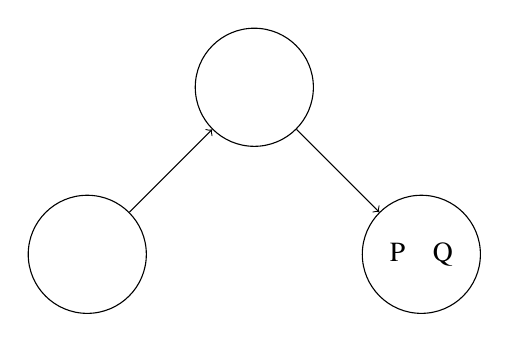
\begin{tikzpicture}[node distance={30mm}, main/.style = {draw, circle, minimum size=15mm}]
            \node[main] (1) {};
            \node[main] (2) [above right of=1] {};
            \node[main] (3) [below right of=2] {P \ \ \ Q};
            \draw[->] (1) -- (2);
            \draw[->] (2) -- (3);
        \end{tikzpicture}
    \end{center}
    The leftmost world does not satisfy either of the two operands of the given disjunction, we can then conclude that the sequent is not a tautology.
\end{enumerate}

\end{document}